\section{Introduction}
	Product Development is driven by stakeholder requirements. The larger the developed system, the harder it is to analyze and verify it. Software Projects are no exceptions. This project aims to show how the verification of huge software projects can be performed automatically against the given requirements.
	
	\begin{figure}[H]
		\centering
		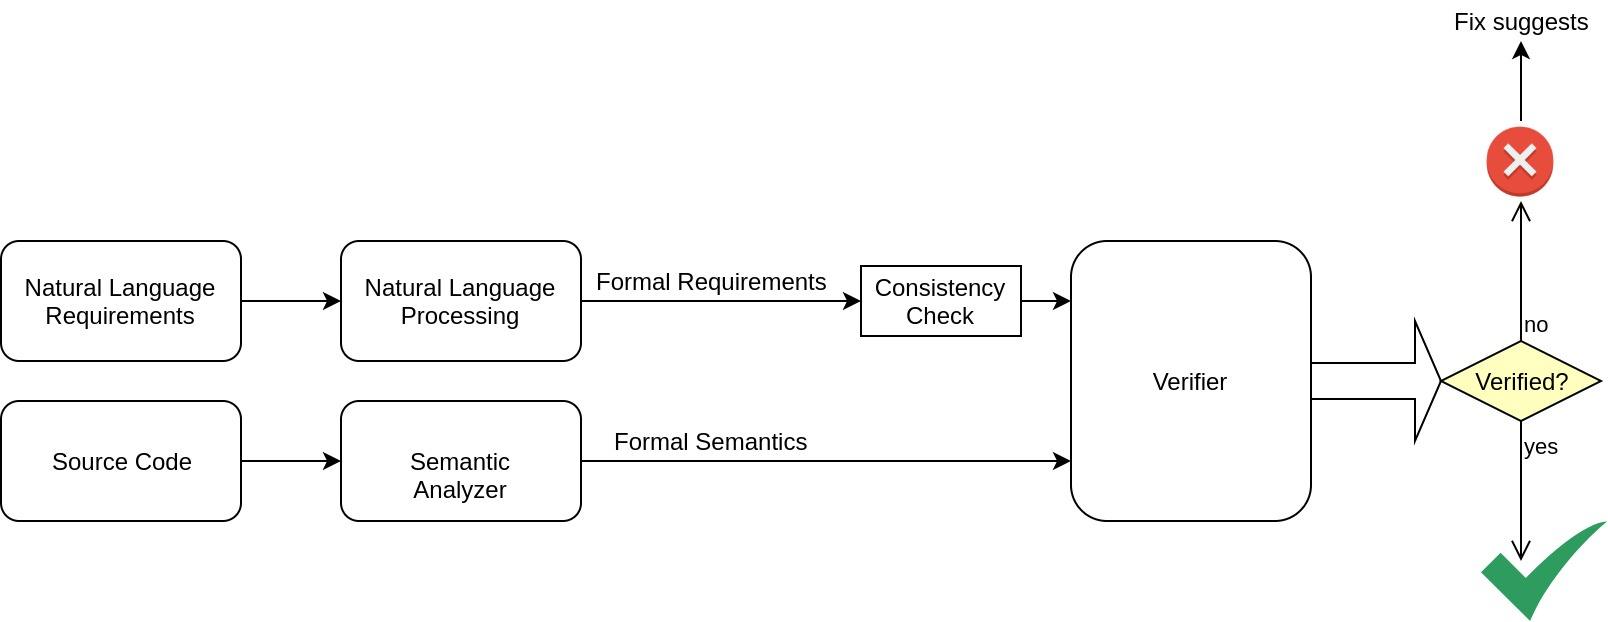
\includegraphics[width=1\linewidth]{../Architecture}
		\caption[PorjArch]{Project Architecture}
		\label{fig:architecture}
	\end{figure}
	
\begin{multicols}{2}	
	\gls{NLP} is used for formalizing the \gls{SRS}. Since, natural language is widely understood by stakeholders, it is used as a common way for representing requirements. Representing requirements in natural language suffers from potential problems like ambiguity, inconsistency and incompleteness.
	
	One of the highest challenge in software engineering is developing software based on unclear requirements. Researches and literature reviews for the last 20 years shows that this is a known problem and big problem \cite{Besrour}. From the very beginning of software engineering, engineers, researchers and scientist used formal and semi-formal methods as a solution of this problem. Yet, initial requirements is written in natural language and there is no escape to avoid it, even by using formal and semi-formal methods \cite{Kamsties}. Moreover, in industrial projects stakeholders usually come from different areas and they may not know formal methods.
	
	Due to unclear requirements the software project development may lead to higher costs and effort, or even a failure in cases where requirements were not understood.
	Common problem, when two software developers interpret requirements differently, based on their point of view. Ferrari et al. (2014) asserted that subjective interpretation leads to software design which is different from the one what was expected in the requirements \cite{Ferrari}.
	
	In the last half century, \gls{SRS} processing and analysis has been one of the focus researching area in software engineering. Due to unclearness of natural language, computer automation of analyzing \gls{SRS} always was a huge challenge. Therefore, the analysis of \gls{SRS} is made manually, what requires time, high costs and effort. But most importantly, as it was mentioned above, the manual analysis of \gls{SRS} leads to imprecise and mistaken results \cite{Wang}. With higher number of requirement (hundreds \gls{SRS} documents containing thousands requirements) this problem will be even more critical and hardly avoidable. Hence, verifying thousands requirements manually by humans will lead to extremely high costs \cite{Fanmuy}.
	
	The importance of finding a way to automate \gls{SRS} processing is unarguably important, roughly, because the main source of problems in requirement engineering is its gross dependence on humans \cite{Ahmed}. As a possible solution to resolve unclearness and provide valuable and clear information to software developers is using \gls{NLP}.
	
	Ryan (1993) questioned that: ”It is highly questionable that the resulting system from \gls{NLP} would be of great use in requirements engineering” \cite{Ryan}.
	
	Nazir et al. (2017) worked on a systematic literature review on \gls{NLP} applications for software requirement engineering and he consummated that: “Manual operations are still required on initial plain text of software requirements before applying the desired \gls{NLP} techniques” \cite{Nazir}.
	
	Besides the \gls{NLP}, our work can create and analyze the formal semantics of the source code.  A formal semantics should serve as a solid foundation for any programming language development, so it must be correct and complete (to be trusted and useful), executable (to yield a reference implementation), and appropriate for program reasoning and verification.
	
	Several efforts to give C a formal semantics have been made, most notably by Charles McEwen Ellison (III.). His executable formal semantics of the C language successfully passes  99.2\% of 776 test programs \cite{Ellison:2012:EFS:2103621.2103719}. Having to define two or more different semantics for a real-life language, together with proofs of equivalence, is a huge burden in itself, not to mention that these all need to be maintained as the language evolves.
	
	Currently code validation falls into two categories: testing and formal verification. Formal verification mainly includes two methods: theorem proving and model checking.
	
	Theorem Proving requires considerable expertise to guide and assist the verification process, and can not generate counter-examples that are useful for debugging when the verification fails.
	
	Model Checking \cite{Clarke:2000:MC:332656} is an automatic formal verification technique for a finite state system, where all the states of the system are exhaustively enumerated and the correctness condition checked at each state. Moreover, model checking yields extremely useful counter examples if it fails. It has proven effective in detecting errors in hardware designs.
	
	Software model checking could produce major enhancements in software reliability and robustness. However, the state space of software programs is typically so huge that they cannot be directly model checked with conventional model checking methods. Fortunately, applying mathematically abstraction methods might extract a reduced model from a program which makes model checking feasible.
	
	Our goal is to tackle multiple problems listed above. Design and train an \gls{NLP} for reliably analyzing the requirements and to verify the semantics of the C source code against the given requirements.
	
\end{multicols}

